\begin{figure}[h!]
  \centering
  \begin{tikzpicture}
    [spy scope= {circle, magnification=6, size=3cm},
      every spy on node/.style={draw, blue, thick},
      every node/.style={inner sep=0},
      label distance=-1cm]

    \node (original) {
      \begin{minipage}{0.35\textwidth}
        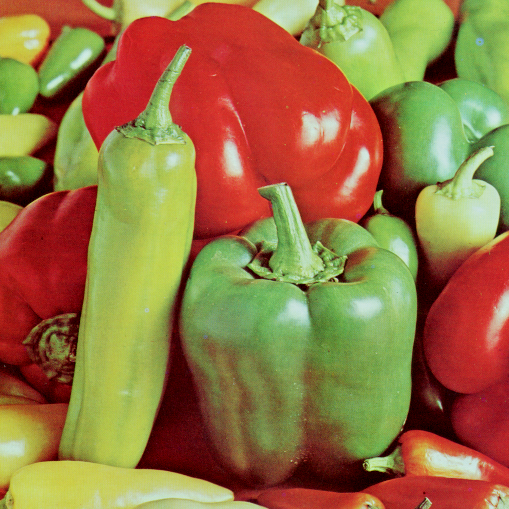
\includegraphics[width=1\textwidth]{peppers/peppers-0.png}
        \caption*{Original}
      \end{minipage}
    };
    \node [right= of original] (300kb) {
      \begin{minipage}{0.35\textwidth}
        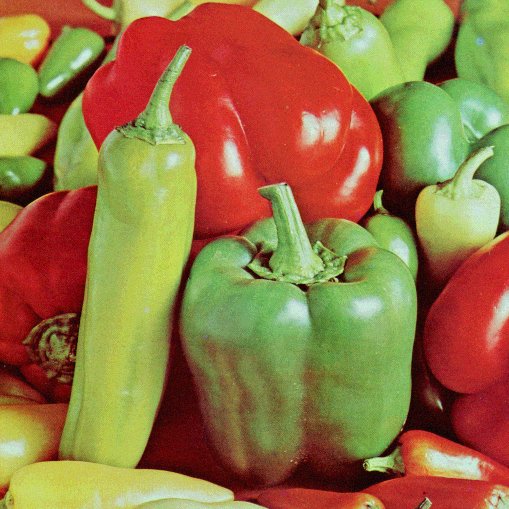
\includegraphics[width=1\textwidth]{peppers/peppers-48.png}
        \caption*{48\,\% (373\,kB)}
      \end{minipage}
    };
    \node [below=0.5cm of original] (500kb) {
      \begin{minipage}{0.35\textwidth}
        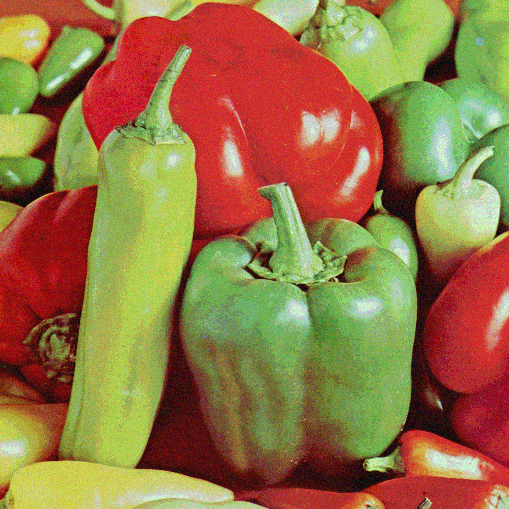
\includegraphics[width=1\textwidth]{peppers/peppers-60.png}
        \caption*{60\,\% (466\,kB)}
      \end{minipage}
    };
    \node [below=0.5cm of 300kb] (700kb) {
      \begin{minipage}{0.35\textwidth}
        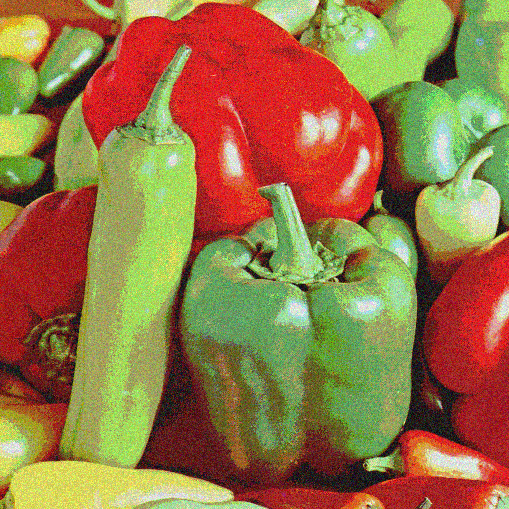
\includegraphics[width=1\textwidth]{peppers/peppers-72.png}
        \caption*{72\,\% (560\,kB)}
      \end{minipage}
    };

    \matrix [column sep=3.5cm] at ($(original.north)!0.5!(300kb.north) + (0,3.5cm)$) {
      \coordinate (a); & \coordinate (b); & \coordinate (c); & \coordinate (d); \\
    };

    \coordinate (spy-on) at (-0.95cm,-0.8cm);

    \spy on ($(original.north) + (spy-on)$) in node[label=below:Original] at (a);
    \spy on ($(300kb.north) + (spy-on)$) in node[label=below:48\,\%] at (b);
    \spy on ($(500kb.north) + (spy-on)$) in node[label=below:60\,\%] at (c);
    \spy on ($(700kb.north) + (spy-on)$) in node[label=below:72\,\%] at (d);


  \end{tikzpicture}
  \caption{Paprika mit einer Größe von 509 $\times$ 509 Pixel.
    Gute Bildqualität zwischen 373 und 466\,kB versteckter Nachricht ($\bmax \approx 777$\,kB).}
  \label{fig:example-peppers}
\end{figure}
